
%% bare_jrnl.tex
%% V1.4b
%% 2015/08/26
%% by Michael Shell
%% see http://www.michaelshell.org/
%% for current contact information.
%%
%% This is a skeleton file demonstrating the use of IEEEtran.cls
%% (requires IEEEtran.cls version 1.8b or later) with an IEEE
%% journal paper.
%%
%% Support sites:
%% http://www.michaelshell.org/tex/ieeetran/
%% http://www.ctan.org/pkg/ieeetran
%% and
%% http://www.ieee.org/

%%*************************************************************************
%% Legal Notice:
%% This code is offered as-is without any warranty either expressed or
%% implied; without even the implied warranty of MERCHANTABILITY or
%% FITNESS FOR A PARTICULAR PURPOSE! 
%% User assumes all risk.
%% In no event shall the IEEE or any contributor to this code be liable for
%% any damages or losses, including, but not limited to, incidental,
%% consequential, or any other damages, resulting from the use or misuse
%% of any information contained here.
%%
%% All comments are the opinions of their respective authors and are not
%% necessarily endorsed by the IEEE.
%%
%% This work is distributed under the LaTeX Project Public License (LPPL)
%% ( http://www.latex-project.org/ ) version 1.3, and may be freely used,
%% distributed and modified. A copy of the LPPL, version 1.3, is included
%% in the base LaTeX documentation of all distributions of LaTeX released
%% 2003/12/01 or later.
%% Retain all contribution notices and credits.
%% ** Modified files should be clearly indicated as such, including  **
%% ** renaming them and changing author support contact information. **
%%*************************************************************************


% *** Authors should verify (and, if needed, correct) their LaTeX system  ***
% *** with the testflow diagnostic prior to trusting their LaTeX platform ***
% *** with production work. The IEEE's font choices and paper sizes can   ***
% *** trigger bugs that do not appear when using other class files.       ***                          ***
% The testflow support page is at:
% http://www.michaelshell.org/tex/testflow/



\documentclass[10pt, onecolumn, twoside, peerreview]{IEEEtran}
\usepackage[letterpaper, margin=0.75in]{geometry}
%
% If IEEEtran.cls has not been installed into the LaTeX system files,
% manually specify the path to it like:
% \documentclass[journal]{../sty/IEEEtran}





% Some very useful LaTeX packages include:
% (uncomment the ones you want to load)


% *** MISC UTILITY PACKAGES ***
%
%\usepackage{ifpdf}
% Heiko Oberdiek's ifpdf.sty is very useful if you need conditional
% compilation based on whether the output is pdf or dvi.
% usage:
% \ifpdf
%   % pdf code
% \else
%   % dvi code
% \fi
% The latest version of ifpdf.sty can be obtained from:
% http://www.ctan.org/pkg/ifpdf
% Also, note that IEEEtran.cls V1.7 and later provides a builtin
% \ifCLASSINFOpdf conditional that works the same way.
% When switching from latex to pdflatex and vice-versa, the compiler may
% have to be run twice to clear warning/error messages.






% *** CITATION PACKAGES ***
%
%\usepackage{cite}
% cite.sty was written by Donald Arseneau
% V1.6 and later of IEEEtran pre-defines the format of the cite.sty package
% \cite{} output to follow that of the IEEE. Loading the cite package will
% result in citation numbers being automatically sorted and properly
% "compressed/ranged". e.g., [1], [9], [2], [7], [5], [6] without using
% cite.sty will become [1], [2], [5]--[7], [9] using cite.sty. cite.sty's
% \cite will automatically add leading space, if needed. Use cite.sty's
% noadjust option (cite.sty V3.8 and later) if you want to turn this off
% such as if a citation ever needs to be enclosed in parenthesis.
% cite.sty is already installed on most LaTeX systems. Be sure and use
% version 5.0 (2009-03-20) and later if using hyperref.sty.
% The latest version can be obtained at:
% http://www.ctan.org/pkg/cite
% The documentation is contained in the cite.sty file itself.






% *** GRAPHICS RELATED PACKAGES ***
%
% \ifCLASSINFOpdf
  % \usepackage{pstricks}
  \usepackage{longtable,tabu}
  \usepackage{graphicx}
  \usepackage{caption}
  % declare the path(s) where your graphic files are
  \graphicspath{{images/}}
  % and their extensions so you won't have to specify these with
  % every instance of \includegraphics
  \DeclareGraphicsExtensions{.JPG,.pdf}
% \else
  % or other class option (dvipsone, dvipdf, if not using dvips). graphicx
  % will default to the driver specified in the system graphics.cfg if no
  % driver is specified.
  % \usepackage[dvips]{graphicx}
  % declare the path(s) where your graphic files are
  % \graphicspath{{../eps/}}
  % and their extensions so you won't have to specify these with
  % every instance of \includegraphics
  % \DeclareGraphicsExtensions{.eps}
% \fi
% graphicx was written by David Carlisle and Sebastian Rahtz. It is
% required if you want graphics, photos, etc. graphicx.sty is already
% installed on most LaTeX systems. The latest version and documentation
% can be obtained at: 
% http://www.ctan.org/pkg/graphicx
% Another good source of documentation is "Using Imported Graphics in
% LaTeX2e" by Keith Reckdahl which can be found at:
% http://www.ctan.org/pkg/epslatex
%
% latex, and pdflatex in dvi mode, support graphics in encapsulated
% postscript (.eps) format. pdflatex in pdf mode supports graphics
% in .pdf, .jpeg, .png and .mps (metapost) formats. Users should ensure
% that all non-photo figures use a vector format (.eps, .pdf, .mps) and
% not a bitmapped formats (.jpeg, .png). The IEEE frowns on bitmapped formats
% which can result in "jaggedy"/blurry rendering of lines and letters as
% well as large increases in file sizes.
%
% You can find documentation about the pdfTeX application at:
% http://www.tug.org/applications/pdftex





% *** MATH PACKAGES ***
%
%\usepackage{amsmath}
% A popular package from the American Mathematical Society that provides
% many useful and powerful commands for dealing with mathematics.
%
% Note that the amsmath package sets \interdisplaylinepenalty to 10000
% thus preventing page breaks from occurring within multiline equations. Use:
%\interdisplaylinepenalty=2500
% after loading amsmath to restore such page breaks as IEEEtran.cls normally
% does. amsmath.sty is already installed on most LaTeX systems. The latest
% version and documentation can be obtained at:
% http://www.ctan.org/pkg/amsmath





% *** SPECIALIZED LIST PACKAGES ***
%
%\usepackage{algorithmic}
% algorithmic.sty was written by Peter Williams and Rogerio Brito.
% This package provides an algorithmic environment fo describing algorithms.
% You can use the algorithmic environment in-text or within a figure
% environment to provide for a floating algorithm. Do NOT use the algorithm
% floating environment provided by algorithm.sty (by the same authors) or
% algorithm2e.sty (by Christophe Fiorio) as the IEEE does not use dedicated
% algorithm float types and packages that provide these will not provide
% correct IEEE style captions. The latest version and documentation of
% algorithmic.sty can be obtained at:
% http://www.ctan.org/pkg/algorithms
% Also of interest may be the (relatively newer and more customizable)
% algorithmicx.sty package by Szasz Janos:
% http://www.ctan.org/pkg/algorithmicx




% *** ALIGNMENT PACKAGES ***
%
%\usepackage{array}
% Frank Mittelbach's and David Carlisle's array.sty patches and improves
% the standard LaTeX2e array and tabular environments to provide better
% appearance and additional user controls. As the default LaTeX2e table
% generation code is lacking to the point of almost being broken with
% respect to the quality of the end results, all users are strongly
% advised to use an enhanced (at the very least that provided by array.sty)
% set of table tools. array.sty is already installed on most systems. The
% latest version and documentation can be obtained at:
% http://www.ctan.org/pkg/array


% IEEEtran contains the IEEEeqnarray family of commands that can be used to
% generate multiline equations as well as matrices, tables, etc., of high
% quality.




% *** SUBFIGURE PACKAGES ***
%\ifCLASSOPTIONcompsoc
%  \usepackage[caption=false,font=normalsize,labelfont=sf,textfont=sf]{subfig}
%\else
%  \usepackage[caption=false,font=footnotesize]{subfig}
%\fi
% subfig.sty, written by Steven Douglas Cochran, is the modern replacement
% for subfigure.sty, the latter of which is no longer maintained and is
% incompatible with some LaTeX packages including fixltx2e. However,
% subfig.sty requires and automatically loads Axel Sommerfeldt's caption.sty
% which will override IEEEtran.cls' handling of captions and this will result
% in non-IEEE style figure/table captions. To prevent this problem, be sure
% and invoke subfig.sty's "caption=false" package option (available since
% subfig.sty version 1.3, 2005/06/28) as this is will preserve IEEEtran.cls
% handling of captions.
% Note that the Computer Society format requires a larger sans serif font
% than the serif footnote size font used in traditional IEEE formatting
% and thus the need to invoke different subfig.sty package options depending
% on whether compsoc mode has been enabled.
%
% The latest version and documentation of subfig.sty can be obtained at:
% http://www.ctan.org/pkg/subfig




% *** FLOAT PACKAGES ***
%
%\usepackage{fixltx2e}
% fixltx2e, the successor to the earlier fix2col.sty, was written by
% Frank Mittelbach and David Carlisle. This package corrects a few problems
% in the LaTeX2e kernel, the most notable of which is that in current
% LaTeX2e releases, the ordering of single and double column floats is not
% guaranteed to be preserved. Thus, an unpatched LaTeX2e can allow a
% single column figure to be placed prior to an earlier double column
% figure.
% Be aware that LaTeX2e kernels dated 2015 and later have fixltx2e.sty's
% corrections already built into the system in which case a warning will
% be issued if an attempt is made to load fixltx2e.sty as it is no longer
% needed.
% The latest version and documentation can be found at:
% http://www.ctan.org/pkg/fixltx2e


%\usepackage{stfloats}
% stfloats.sty was written by Sigitas Tolusis. This package gives LaTeX2e
% the ability to do double column floats at the bottom of the page as well
% as the top. (e.g., "\begin{figure*}[!b]" is not normally possible in
% LaTeX2e). It also provides a command:
%\fnbelowfloat
% to enable the placement of footnotes below bottom floats (the standard
% LaTeX2e kernel puts them above bottom floats). This is an invasive package
% which rewrites many portions of the LaTeX2e float routines. It may not work
% with other packages that modify the LaTeX2e float routines. The latest
% version and documentation can be obtained at:
% http://www.ctan.org/pkg/stfloats
% Do not use the stfloats baselinefloat ability as the IEEE does not allow
% \baselineskip to stretch. Authors submitting work to the IEEE should note
% that the IEEE rarely uses double column equations and that authors should try
% to avoid such use. Do not be tempted to use the cuted.sty or midfloat.sty
% packages (also by Sigitas Tolusis) as the IEEE does not format its papers in
% such ways.
% Do not attempt to use stfloats with fixltx2e as they are incompatible.
% Instead, use Morten Hogholm'a dblfloatfix which combines the features
% of both fixltx2e and stfloats:
%
% \usepackage{dblfloatfix}
% The latest version can be found at:
% http://www.ctan.org/pkg/dblfloatfix




%\ifCLASSOPTIONcaptionsoff
%  \usepackage[nomarkers]{endfloat}
% \let\MYoriglatexcaption\caption
% \renewcommand{\caption}[2][\relax]{\MYoriglatexcaption[#2]{#2}}
%\fi
% endfloat.sty was written by James Darrell McCauley, Jeff Goldberg and 
% Axel Sommerfeldt. This package may be useful when used in conjunction with 
% IEEEtran.cls'  captionsoff option. Some IEEE journals/societies require that
% submissions have lists of figures/tables at the end of the paper and that
% figures/tables without any captions are placed on a page by themselves at
% the end of the document. If needed, the draftcls IEEEtran class option or
% \CLASSINPUTbaselinestretch interface can be used to increase the line
% spacing as well. Be sure and use the nomarkers option of endfloat to
% prevent endfloat from "marking" where the figures would have been placed
% in the text. The two hack lines of code above are a slight modification of
% that suggested by in the endfloat docs (section 8.4.1) to ensure that
% the full captions always appear in the list of figures/tables - even if
% the user used the short optional argument of \caption[]{}.
% IEEE papers do not typically make use of \caption[]'s optional argument,
% so this should not be an issue. A similar trick can be used to disable
% captions of packages such as subfig.sty that lack options to turn off
% the subcaptions:
% For subfig.sty:
% \let\MYorigsubfloat\subfloat
% \renewcommand{\subfloat}[2][\relax]{\MYorigsubfloat[]{#2}}
% However, the above trick will not work if both optional arguments of
% the \subfloat command are used. Furthermore, there needs to be a
% description of each subfigure *somewhere* and endfloat does not add
% subfigure captions to its list of figures. Thus, the best approach is to
% avoid the use of subfigure captions (many IEEE journals avoid them anyway)
% and instead reference/explain all the subfigures within the main caption.
% The latest version of endfloat.sty and its documentation can obtained at:
% http://www.ctan.org/pkg/endfloat
%
% The IEEEtran \ifCLASSOPTIONcaptionsoff conditional can also be used
% later in the document, say, to conditionally put the References on a 
% page by themselves.




% *** PDF, URL AND HYPERLINK PACKAGES ***
%
%\usepackage{url}
% url.sty was written by Donald Arseneau. It provides better support for
% handling and breaking URLs. url.sty is already installed on most LaTeX
% systems. The latest version and documentation can be obtained at:
% http://www.ctan.org/pkg/url
% Basically, \url{my_url_here}.




% *** Do not adjust lengths that control margins, column widths, etc. ***
% *** Do not use packages that alter fonts (such as pslatex).         ***
% There should be no need to do such things with IEEEtran.cls V1.6 and later.
% (Unless specifically asked to do so by the journal or conference you plan
% to submit to, of course. )


% correct bad hyphenation here
\hyphenation{op-tical net-works semi-conduc-tor}

% *** CUSTOM CODE ***
% This brings in the listings package and color package so we can include code snippets into our document.
% The additional code after that is to define the Javascript language because listings doesn't have a 
% definition for Javascript.
\usepackage{listings}
\usepackage{color}
\usepackage{hyperref}
\definecolor{lightgray}{rgb}{.9,.9,.9}
\definecolor{darkgray}{rgb}{.4,.4,.4}
\definecolor{purple}{rgb}{0.65, 0.12, 0.82}
\lstdefinelanguage{JavaScript}{
  keywords={break, case, catch, continue, debugger, default, delete, do, else, false, finally, for, function, if, in, instanceof, new, null, return, switch, this, throw, true, try, typeof, var, void, while, with},
  morecomment=[l]{//},
  morecomment=[s]{/*}{*/},
  morestring=[b]',
  morestring=[b]",
  ndkeywords={class, export, boolean, throw, implements, import, this},
  keywordstyle=\color{blue}\bfseries,
  ndkeywordstyle=\color{darkgray}\bfseries,
  identifierstyle=\color{black},
  commentstyle=\color{purple}\ttfamily,
  stringstyle=\color{red}\ttfamily,
  sensitive=true
}

\lstset{
   language=JavaScript,
   backgroundcolor=\color{lightgray},
   extendedchars=true,
   basicstyle=\footnotesize\ttfamily,
   showstringspaces=false,
   showspaces=false,
   numbers=left,
   numberstyle=\footnotesize,
   numbersep=9pt,
   tabsize=2,
   breaklines=true,
   showtabs=false,
   captionpos=b
}

\begin{document}
%
% paper title
% Titles are generally capitalized except for words such as a, an, and, as,
% at, but, by, for, in, nor, of, on, or, the, to and up, which are usually
% not capitalized unless they are the first or last word of the title.
% Linebreaks \\ can be used within to get better formatting as desired.
% Do not put math or special symbols in the title.
\title{Silicon Tracking Solutions}
%
%
% author names and IEEE memberships
% note positions of commas and nonbreaking spaces ( ~ ) LaTeX will not break
% a structure at a ~ so this keeps an author's name from being broken across
% two lines.
% use \thanks{} to gain access to the first footnote area
% a separate \thanks must be used for each paragraph as LaTeX2e's \thanks
% was not built to handle multiple paragraphs
%

\author{Brett~Hayes,
        Joseph~Cronise,
        and~Dylan~Camus\\% <-this % stops a space
        CS463~/~Spring~2016~/~Group 03\\% <-this % stops a space
        Final~Report
\thanks{CS463/ Spring 2016 / Group 03}% <- this % stops a space
\thanks{Final Report}}


% note the % following the last \IEEEmembership and also \thanks - 
% these prevent an unwanted space from occurring between the last author name
% and the end of the author line. i.e., if you had this:
% 
% \author{....lastname \thanks{...} \thanks{...} }
%                     ^------------^------------^----Do not want these spaces!
%
% a space would be appended to the last name and could cause every name on that
% line to be shifted left slightly. This is one of those "LaTeX things". For
% instance, "\textbf{A} \textbf{B}" will typeset as "A B" not "AB". To get
% "AB" then you have to do: "\textbf{A}\textbf{B}"
% \thanks is no different in this regard, so shield the last } of each \thanks
% that ends a line with a % and do not let a space in before the next \thanks.
% Spaces after \IEEEmembership other than the last one are OK (and needed) as
% you are supposed to have spaces between the names. For what it is worth,
% this is a minor point as most people would not even notice if the said evil
% space somehow managed to creep in.



% The paper headers
\markboth{Final Report \today}%
{Silicon Tracking Solutions}%{Shell \MakeLowercase{\textit{et al.}}: Bare Demo of IEEEtran.cls for IEEE Journals}
% The only time the second header will appear is for the odd numbered pages
% after the title page when using the twoside option.
% 
% *** Note that you probably will NOT want to include the author's ***
% *** name in the headers of peer review papers.                   ***
% You can use \ifCLASSOPTIONpeerreview for conditional compilation here if
% you desire.




% If you want to put a publisher's ID mark on the page you can do it like
% this:
%\IEEEpubid{0000--0000/00\$00.00~\copyright~2015 IEEE}
% Remember, if you use this you must call \IEEEpubidadjcol in the second
% column for its text to clear the IEEEpubid mark.



% use for special paper notices
%\IEEEspecialpapernotice{(Invited Paper)}




% make the title area
\maketitle

% As a general rule, do not put math, special symbols or citations
% in the abstract or keywords.
\begin{abstract}
This document contains the work of Brett Hayes, Joseph Cronise, and Dylan Camus pertaining to the Silicon Tracking
project. This project is a web-based inventory system used by the Performance, Measurement, and Analysis team at Intel
in Chandler, AZ. The inventory system we have designed tracks the information and status of CPU silicon used by the
team and is made to help them to know where their high value inventory is at all times, as well as saving the team time
and effort towards obtaining the items they need to get their work done. We have designed for them a system such that
every time an engineer within their lab needs to use an item, they will need to check out the item through our system
and check it back in when they are done. This ensures that highly sensitive materials don’t go missing without a log of
who has had ownership of the item, as well as letting others know who currently is in ownership of the item.
\end{abstract}

% Note that keywords are not normally used for peerreview papers.
% \begin{IEEEkeywords}
% IEEE, IEEEtran, journal, \LaTeX, paper, template.
% \end{IEEEkeywords}






% For peer review papers, you can put extra information on the cover
% page as needed:
 \ifCLASSOPTIONpeerreview
 % \begin{center} \bfseries EDICS Category: 3-BBND \end{center}
 \fi
%
% For peerreview papers, this IEEEtran command inserts a page break and
% creates the second title. It will be ignored for other modes.
\IEEEpeerreviewmaketitle



\section{Introduction} 
% The very first letter is a 2 line initial drop letter followed % by the rest of the first word in caps. %
% form to use if the first word consists of a single letter: % \IEEEPARstart{A}{demo} file is .... %
% form to use if you need the single drop letter followed by % normal text (unknown if ever used by the IEEE): %
% \IEEEPARstart{A}{}demo file is .... %
% Some journals put the first two words in caps: 
% \IEEEPARstart{T}{his demo} file is .... %
% Here we have the typical use of a "T" for an initial drop letter % and "HIS" in caps to complete the first word. 
\IEEEPARstart{T}{he} Lorem ipsum dolor sit amet, consectetur adipiscing elit. Morbi viverra tortor at nunc tristique,
et faucibus magna tempus. Vestibulum elementum dolor in porttitor facilisis. Vivamus commodo nibh nulla, eget suscipit
felis tincidunt sed. Proin ut metus diam. Phasellus consectetur congue elit, quis vehicula nunc facilisis quis. Morbi
dapibus risus vitae felis blandit pulvinar. Maecenas fringilla leo sed dictum pulvinar. Sed tempus, felis vel tincidunt
varius, dui nulla laoreet orci, vel accumsan magna erat sed est. Aenean luctus quam a feugiat malesuada. Duis viverra
lectus purus, id malesuada risus bibendum at. Aenean malesuada, magna id facilisis dapibus, leo nulla fermentum elit,
nec imperdiet purus nisi non arcu. Suspendisse placerat, est nec feugiat tincidunt, ex risus dictum ante, id dignissim
lectus lorem vitae odio. Fusce ac quam ut arcu porta ultrices. Quisque porta volutpat tortor, ut ultricies velit
viverra eget.\\

Nulla facilisi. Donec cursus sodales est, quis eleifend urna congue sit amet. Nunc accumsan, mi sed dapibus convallis,
nunc felis auctor libero, a maximus nulla mauris ut enim. Vivamus vulputate ipsum odio, vel tincidunt leo aliquam in.
In varius urna quis purus iaculis aliquam. Donec egestas lectus vitae justo dapibus, et pharetra risus lobortis. Nullam
pulvinar justo ut purus efficitur ornare. Proin rutrum dictum purus eget vehicula.\\

Proin ut ipsum ante. Nulla porttitor eros at metus pretium viverra. Vestibulum ut elit at dui accumsan convallis ac vel
mauris. Cras venenatis ante ac arcu volutpat vehicula. Nullam id tortor vitae augue interdum ultricies. Cras pharetra
elit sed viverra scelerisque. Aenean cursus nulla ut arcu posuere hendrerit. Vestibulum ante ipsum primis in faucibus
orci luctus et ultrices posuere cubilia Curae; Integer ipsum libero, tempor et ornare in, facilisis vel ex. Integer
eget leo facilisis erat euismod rhoncus. Quisque sapien quam, dictum vitae arcu id, posuere aliquet lacus. Phasellus
porttitor tortor metus, eu vehicula eros condimentum et. Praesent odio justo, sagittis id vestibulum sed, posuere sit
amet neque.\\

Integer et ornare orci. Aliquam eget ligula et tortor finibus condimentum. Quisque at tempor risus. Vivamus fringilla
lobortis eros, nec eleifend sapien lacinia eu. Mauris interdum pulvinar nisl vel aliquam. In eget nibh id risus aliquam
efficitur. Vestibulum gravida ante quis tortor placerat dapibus. Aliquam dignissim vestibulum tempor. Integer nec porta
sem, et egestas libero. Nam vel nisl quis nulla volutpat pretium. Aliquam luctus laoreet imperdiet.\\

% You must have at least 2 lines in the paragraph with the drop letter
% (should never be an issue)

\section{The Original Requirements Document}
This is the Requirements Document we wrote at the beginning of the
project. It has been re-formatted to keep consistent styling across the document, but the content of the document has
not been modified. We have also indexed the requirements in this document for easy reference. The original document in its original formatting is included on the usb storage drive.
\subsection{Introduction}

\subsubsection{About This Document}
This is the requirements document for the Silicon Tracker project. Included in the following sections are lists of user
stories organized by categories. Each paragraph contains a feature to be added to the web application. They are all
organized into their respective categories and are set up as individual tasks to be checked off as they are
completed.\\

\subsubsection{Definitions}
The “kiosk” mentioned in a few user stories is a nickname that the Intel PMA Labs has given for their check in/check
out system. They have a computer with a QR scanner that sits on top of a large locker with all the items they store.\\

Although one of the main items being tracked will be silicon, we use the generic term “item” to specify that any part
needed, not just silicon, can be inventoried by our system.\\

\subsubsection{Current System}
The current system Intel uses is inadequate for their needs. The items have to be checked in or out one at a time. This
means the user has to enter their credentials for every item that goes through the system. They are wanting a more
user-friendly web application where they can add items to their “shopping cart” and when they are ready, go to the
kiosk and check in and out all their items in a single transaction.\\

\subsection{The Client would like to...}

\subsubsection{Inventory}
\paragraph*{Req 1} Queue an item that the user wants but is not checked in. If a person needs this item and it is currently checked out,
they can be put on a queue for that item.\\

\paragraph*{Req 2} Give a reason and a priority when queueing an item. This will create a priority queue for the users. If someone needs
an item and it is important, they can give a reason why.\\

\paragraph*{Req 3} When an item gets checked in and there were people waitlisting on the item, the people who have waitlisted will be
notified with everyone's priority and reason for needing the item.\\

\paragraph*{Req 4} Check out an item that is checked into the system. If nobody else has the item reserved, they can check out the item
immediately.\\

\paragraph*{Req 5} Check in an item that was checked out of the system. The user returns the item so other people can check out the
item.\\

\paragraph*{Req 6} Check in multiple items in a single transaction. The current system doesn’t allow this feature. This would let the user
check in multiple items without giving their credentials for every item.\\

\paragraph*{Req 7} Check out multiple items in a single transaction. The current system doesn’t allow this feature. This would let the
user check out multiple items without giving their credentials for every item.\\

\paragraph*{Req 8} Check in and check out multiple items in the same transaction. Along with the above two stories, the user should be
able to both check in and out and only give their credentials once.\\

\paragraph*{Req 9} Enter new items into the system. There should be a form that a user can fill out. They will scan the item to insert the
item’s ID.\\

\paragraph*{Req 10} Retire old items in the system. They need to logically delete (scrap) items when an item is no longer being used. There
should be a textbox to optionally give a reason for the item being retired.\\

\paragraph*{Req 11} Be able to scan an item when checking in and have that automatically update the database. The user should just be able
to log in, and then scan the item. The status of the item should be updated based on the item being scanned. This
should happen when the user has the item currently checked out.\\

\paragraph*{Req 12} Be able to scan an item when checking out have that automatically update the database. The user should just be able to
log in, and then scan the item. The status of the item should be updated based on the item being scanned. This should
happen when the user has the item.\\

\paragraph*{Req 13} Be able to scan an item that is currently checked in to see who has the item reserved next. This will show the next
person in line for the item.\\

\paragraph*{Req 14} Be able to scan an item that is currently checked out to see who has the item checked out. For example, if there is an
item that someone left out and nobody knows who has it checked out, the item can be scanned to see who it currently
belongs to.\\

\paragraph*{Workflow of the system}

\paragraph*{Req 15} The initial screen is a welcome screen. This is where the user can scan their badge, use facial recognition, or enter a
username/password to login. After proper authorization, the user is presented with the shopping cart interface.\\

\paragraph*{Req 16} The user can now start scanning items.\\

\paragraph*{Req 17} If the item is scanned and the item is checked in, it will now be checked out by the user. If the item was already
checked out, information about who currently has the item checked out will be displayed on the screen.\\

\paragraph*{Req 18} If the current user has an item checked out, they can scan the item and the item will be checked in.\\

\paragraph*{Req 19} When the user is done, they will press a confirm button and will be shown a list of items they have checked in/out. The
user can then proceed to commit their transaction to the database.\\

\subsubsection{Security}
\paragraph*{Req 20} Log into the application with a username and password.\\

\paragraph*{Req 21} User settings and permissions will be maintained in the project database. Authenticate user credentials using the
Active Directory server already set up at Intel. They already have a system in place and the users will have to sign in
with their current credentials.\\

\paragraph*{Req 22} Authenticate facial recognition using the project database. The data stored for facial recognition will have to be in
the project database, since we cannot modify the Active Directory server.\\

\paragraph*{Req 23} When setting up facial recognition for a user, authenticate user with username and password, or with RFID tag first.
This is for security reasons, so other people won’t try to scan their face on someone else’s profile. When checking in
or out item(s), the user should be able to authenticate with their current RFID tags using an RFID reader.\\

\paragraph*{Req 24} When checking in or out item(s), the user should be able to authenticate with facial recognition.\\

\paragraph*{Req 25} When checking in or out item(s), the user should be able to authenticate with username and password.\\

\paragraph*{Req 26} Those with elevated permissions can retire old items from the system. This will be a logical delete, not an actual
delete from the database.\\

\paragraph*{Req 27} Those with elevated permissions can modify certain fields of the items.\\

\paragraph*{Req 28} Have any communication between the web server and the client will be encrypted through SSL. The information about the
items are all confidential, and they need to stay that way.\\

\paragraph*{Req 29} Admins will have the ability to enable/disable any of the three authentication methods (username/password, RFID tag, or
facial recognition). If for whatever reason the admin does not want one of these methods available, they can disable
that method of authentication.\\

\subsubsection{Database}
\paragraph*{Req 30} Have new items be inserted into the project database.\\

\paragraph*{Req 31} Have old items continue to be stored in the database after they are retired (logically deleted). Certain users still
need the information about items even if they are no longer active.\\

\paragraph*{Req 32}  Have a record of who checked in which items, and have that stored in the database. This creates an audit trail for all
the items.\\

\paragraph*{Req 33} Have a record of who checked out which items, and have that stored in the database. This creates an audit trail for all
the items.\\

\paragraph*{Req 34} Have a timestamp for every time an item is inserted, updated, or retired. This is also for auditing reasons.\\

\subsubsection{Services}
\paragraph*{Req 35} Have an e-mail sent out when an item is queued to any person that has the specific item checked out.\\

\paragraph*{Req 36} Send out periodic schedulable reports via e-mail to each user based on the items they checked in and out, and have on
queue.\\

\paragraph*{Req 37} Have users be notified via e-mail when they check in an item. This should happen for every transaction, so the user
doesn’t get a separate e-mail for every item.\\

\paragraph*{Req 38} Have users be notified via e-mail when they check out an item. This should happen for every transaction, so the user
doesn’t get a separate e-mail for every item.\\

\paragraph*{Req 39} Have users be notified when an item is now considered retired and they have the item currently checked out. They will
need the e-mail so they know to return it immediately.\\

\subsection{The Interfaces...}
\subsubsection{Main Interface}
\paragraph*{Req 40} Will be a touch interface without need of keyboard. The keyboard will still be available for certain functions, such as
entering a new item. The idea is that the user doesn’t have to use the keyboard for check-in and check-out
transactions.\\

\paragraph*{Req 41} Will be able to check in items from this interface. This should not require a keyboard. The user should simply login to
the system and scan the item(s) to check them in.\\

\paragraph*{Req 42} Will be able to check out items from this interface. This should not require a keyboard. If they have the item ready
for check out, then they should simply login to the system and scan the item(s) to check them out.\\

\paragraph*{Req 43} Will be able to scan an item and display the information about that item (i.e. in the case of silicon, Core Count, LLC
Size, Frequency, Status (Checked in or Checked out), etc.)\\

\subsubsection{Shopping Cart Interface}
\paragraph*{Req 44} Will be able to check in items from this interface. If they are at the kiosk they should have a way to check in items
using this interface.\\

\paragraph*{Req 45} Will be able to check out items from this interface.\\

\paragraph*{Req 46} Will be able to add new items to the system from this interface. When a new item comes in, they will need to enter
information about the item, and then scan it so they have the serial number recorded.\\

\paragraph*{Req 47} Will be able to retire items from circulation (with elevated privileges). The items will be scrapped, but still in the
database for record keeping.\\

\paragraph*{Req 48} Will be able to reuse information of items when the same item is being added to the inventory system. They will have
multiples of the same item. That item should just be scanned and linked with the other items in the system.\\

\paragraph*{Req 49} Will be able to search for items based on certain fields in the database. The user should be able to filter their
search results based on the item attributes.\\

\paragraph*{Req 50} Will have multi-level filtering on searches. For more information, see Appendix – Multi-Level Filtering.\\

\subsubsection{Scrapping Interface}
\paragraph*{Req 51} If a user has the right elevated privileges, they can be taken to a scrapping interface. This interface will be similar
to the shopping cart interface. The difference will lie in the fact that any item the user scans will be scrapped
instead of checked in/out. They will confirm and commit their transaction, just like the shopping cart interface.\\

\subsubsection{Reporting Interface}
\paragraph*{Req 52} Will be able to view any item in circulation. This should be in the form of a user-friendly table with pagination.\\

\paragraph*{Req 53} Will be able to view any item that is retired. This should also be in the form of a user-friendly table with
pagination.\\

\paragraph*{Req 54} Will be able to see what items a certain user has checked out. They should be able to click on a user, and it will give
a list of items in a user-friendly table with pagination.\\

\paragraph*{Req 55} Will be able to search for any user who checked out a certain item. This will display as a table with the users who
have one or more of these items.\\

\paragraph*{Req 56} Will have multi-level filtering on searches. For more information, see Appendix A – Multi-Level Filtering.\\

\subsection{The Expo Should Look Like...}
\subsubsection{Web Application}
\paragraph*{Req 57} A Fully functioning version will be running during the event. This will be a system that the general audience can view
and play with.\\

\paragraph*{Req 58} Anybody can have their faces entered into the database. This will show how the facial recognition works.\\

\paragraph*{Req 59} Anybody can scan sample RFID cards to check in or out items. We will have sample items for them to scan, and they can
use fake RFID badges to simulate the experience.\\

\paragraph*{Req 60} Anybody can scroll through the different interfaces. They will have admin privileges so they can see all the features
of the application.\\

\paragraph*{Req 61} Anybody can check in or out items into the system. There will be a set of sample items people can scan so they can see
how the system works.\\

\subsection{Appendix}
\subsubsection{Multi-Level Filtering}
This is a filtering process for items that are in the database system. It is used for easy search filtering based on
multiple fields. For example, if the user is filtering items based on clock speed and they want to narrow their search
further, then they can select another field to filter on. If they decide to filter again on cache size, then they will
only see the possible filters for cache size based on the items with the specific clock speed they chose earlier.\\

\subsubsection{Gantt Chart}
\begin{figure}[H]
	\includegraphics[angle=90, width=\textwidth]{gantt}
\end{figure}
\clearpage

\section{Project Changes Since the Original Client Requirements Document}

\begin{center}
	\begin{longtabu} to \textwidth {|X[1,l]|X[10,l]|X[10,l]|X[10,l]|}
		\hline
		\# & Requirement & Reason For Changes & Comments \\ \hline
		2 & Give a reason and a priority when queueing an item. This will create a priority queue for the users. If someone needs an item and it is important, they can give a reason why. & Our client stated that since they are a small team, they only needed an email stating that the item has been checked in. All the people can meet up and talk about who gets the item next. & \\ \hline
		10 & Retire old items in the system. They need to logically delete (scrap) items when an item is no longer being used. There should be a textbox to optionally give a reason for the item being retired. & There is no textbox to give a reason for the item being scrapped. Each item has a notes field, and we decided that the best option was to place the reason for scrapping in the item’s notes field. & \\ \hline
		13 & Be able to scan an item that is currently checked in to see who has the item reserved next. This will show the next person in line for the item. & We decided not to be concerned about this, because everyone who reserved an item will discuss in person who needs the item next. & \\ \hline
		17 & If the item is scanned and the item is checked in, it will now be checked out by the user. If the item was already checked out, information about who currently has the item checked out will be displayed on the screen. & Our client asked if we could make it so one person can check in another’s item. & \\ \hline
		19 & When the user is done, they will press a confirm button and will be shown a list of items they have checked in/out. The user can then proceed to commit their transaction to the database. & We made it so they only need to press one button to commit their transaction. A message appears now to just show what items they checked in/out, after they have committed. & \\ \hline
		29 & Admins will have the ability to enable/disable any of the three authentication methods (username/password, RFID tag, or facial recognition). If for whatever reason the admin does not want one of these methods available, they can disable that method of authentication. & Our client’s team implemented RFID security, and the facial recognition was implemented very late in the development phase of the project, so we didn’t get a chance to implement this setting. & \\ \hline
		N/A & The Interfaces & In our original Requirements Document, we had four interfaces. After starting work on this project, we simplified the system down to two interfaces. It made the system easier to discuss and navigate. We boiled down the interfaces into the Web interface and the Kiosk interface. The Shopping Cart interface, Scrapping interface, and Reporting interface have mostly been combined into the Web interface. The Main Interface has mostly been reworked into the Kiosk interface. & All of the requirements within the Interfaces section have been fulfilled, but not necessarily in all of the interfaces specified. \\ \hline
		44 \& 45 & Will be able to check in items from this interface. If they are at the kiosk they should have a way to check in items using this interface. Will be able to check out items from this interface. & Our client let us know that they only need to check in and check out items from one interface. Our original Requirements Document had checking in and out of items from two interfaces. We removed the Checking in and out requirements to allow for these features to happen in only one place. & \\ \hline
		59 & Anybody can scan sample RFID cards to check in or out items. We will have sample items for them to scan, and they can use fake RFID badges to simulate the experience. & Our client’s team implemented the RFID readers, so we did not show how they worked at expo. & \\ \hline
		N/A & New Requirement: Sanitizing and Validation User Input & We did not place in our original document to clean up any user input and make sure that their input is valid. It was an important feature, and our client did ask that we created a system where data entered would be consistent. & \\ \hline
		N/A & New Requirement: Editing Dropdown Menu Items & We setup a page for the admins to change the dropdown menu items. These dropdowns are found when inserting or editing an item. Our client liked the idea of not having to make edits directly in the database, so we implemented this feature. & \\ \hline
		N/A & New Requirement: Quick Check in/out. & We added an extra feature for when a user scans an item to get the item's information, they can click a Check In/Out button to save the item for later. It makes it easier for the user to check in or out an item as soon as they scan it, and makes the workflow a little smoother. & Our client's team received this feature very well and were thankful to have it. \\ \hline
	\end{longtabu}
\end{center}

\section{Describe Any Problems that Have Impeded Your Progress, With Any
Solutions You Have}

We have talked about a few of our blockers in the previous
sections. For instance there is the issue of facial recognition. The other main
issue is with authentication. These two main issues come from the security
concerns and policies at Intel, and hardware issues that we are currently dealing with.\\

There is not really a way for us to get access to how Intel authenticates its
users. So the best that we can do with authentication is come up with our own
version of authentication and try to make it as close to how we believe their
system works. As mentioned earlier, we have created such a system that handles
authentication. It's a server that accepts web requests, and returns a WWID
upon successful authentication. The only real information that we know about
their authentication system is that our application will need to interact with
their authentication server through a web request. Our service does exactly
this. We have been as clear as possible in our code, because the employees at
Intel will have to modify this portion of our code in order to make it work on
their system. We thoroughly commented our code, and I have written to our
client a detailed explanation of how we designed our authentication.\\

A smaller problem that we have been faced with is that we only have sample data
for CPUs. All the other items behave almost identically. They will have a
barcode to be scanned, and will check in and check out through the same methods
as the CPU. This is not a big issue, we just can't test any other items besides
CPU, unless we take a CPU and put it in the system as another item.\\

Whenever we need to use the barcode scanner, we have to go to the capstone lab
on campus. This was a little frustrating, especially when going to the capstone
lab was not an option. To remedy this, we came up with a program that simulates
our barcode scanner. It's a small python script that behaves in the same way as
our scanner when you give it a serial number. This has allowed us to develop
features for the barcode scanner without even using the scanner!

\clearpage

\section{Include Any Particularly Interesting Pieces of Code}
This is an example of some of our back-end code. We are using express.js for our back-end. Express is a package of node.js, a lightweight, asynchronous, open-source runtime environment in JavaScript. This example is showing when a user makes a POST request to the server, when the user adds a new CPU item. The server responds anytime there is a POST request to the URI "/add/cpu". The server first sanitizes the input with our scrub library, and then checks user input with the validation library. If the validator returns with errors, the server sends the error messages back to the web interface. Only when the validator approves of the input does the server make a database call. With valid input, the server makes a call to the database for a stored procedure, which will insert the CPU information into the database.
\begin{lstlisting}[language=Javascript, caption=Server-side Request Handler]
  app.post('/add/cpu', function(req, res) {
    req.body = scrub.CPU(req.body);
    var verrors = validate.CPU(req.body);

    if (verrors) {
      res.status(400).send(verrors);
    } else {
      pool.getConnection(function(err, conn) {
        conn.query("CALL check_serial_cpu('"+req.body.serial_num+"');",
          function(error, results, fields){
            if(error) {
              throw error;
            }
            
            if(results[0].length == 0) {
              conn.query("CALL put_cpu('"+req.body.serial_num+"','"
                +req.body.spec+"','"+req.body.mm+"','"
                +req.body.frequency+"','"+req.body.stepping+"','"
                +req.body.llc+"','"+req.body.cores+"','"
                +req.body.codename+"','"+req.body.cpu_class+"','"
                +req.body.external_name+"','"+req.body.architecture+"','"
                +req.body.notes+"');",
              function(error, results, fields){
                if(error) {
                  throw error;
                }
              });
            }
            conn.release();
            res.status(200).send(req.body);
        });
      });
    } 
  });
\end{lstlisting}

The following code below shows how we implemented the barcode scanner. This
code runs on the kiosk interface in the login page. It is continuously
listening for keyboard input. The way the barcode scanner works is it acts like
a keyboard. When it scans an item, it "types" in the letters of the serial
number one at a time. We came up with an idea that if the barcode types faster
than what is humanly possible, we should be able to decipher between a barcode
scan and a human typing. Once some keyboard input comes in, our code starts a
timer. The code will push all the keys pressed into an array. If there are ten
key presses within 250 milliseconds, we will know that it is a barcode scan
instead of a human typing! Once an item is scanned, it requests from the server
information about the item just scanned. Once information is returned to the
client, it displays the item information on the screen.
\begin{lstlisting}[language=Javascript, caption=Barcode Scanner Listener]
$(window).keypress(function(e) {
      chars.push(String.fromCharCode(e.which));
      if (pressed == false) {
          setTimeout(function(){
              // If there are ten characters inserted before the timeout
              if (chars.length >= 10) {
                  var barcode = chars.join("");
                  // There was an item scanned. Enter response code here.
                  var itemInfo = "";
                  $.get('/serial/'+barcode, function(data) {
                    if (data.item_type === 'cpu') {$('#item-info').html(CPUInfo(data));}
                    else if (data.item_type === 'ssd') {$('#item-info').html(SSDInfo(data));}
                    else if (data.item_type === 'memory') {$('#item-info').html(MemoryInfo(data));}
                    else if (data.item_type === 'flash_drive') {$('#item-info').html(FlashDriveInfo(data));}
                    else if (data.item_type === 'board') {$('#item-info').html(BoardInfo(data));}
                    else {$('#item-info').html(ErrorInfo());}
                  });
              }
              chars = [];
              pressed = false;
          },250); // <-- this is the timeout in milliseconds
      }
      pressed = true;
  });
\end{lstlisting}

\section{User Studies}
We continually talk with our client about the project and how it is working out
for them. Our highest priority is to make sure that they are happy with the
work we produce.\\

Since our code is on our repository on-line, they have access to our project in
its current state. They have two instances of an inventory system right now.
One instance is their old inventory system. The other instance is our inventory
system in its current state. Our client has asked his team to use both
inventory systems when checking in and out items. This gives us a lot of
feedback on how our system is working in the intended environment, and we are
taking all of their feedback into consideration.\\

A lot of the feedback we get pertains to bug fixes. Some of the bugs are
specific to their setup, and we would have never known about if they weren't
actively using it. For instance, with their system they have their server and
database running on separate machines. If the server has not made any requests
in a specified amount of time, the database will close the connection with the
server. They would have to restart the server in order to get the connection
back with the database. On our development environment, we have the server and
database running on the same machine, so there is never a connection issue
between the two.\\

We are constantly receiving positive feedback from our client and his team.
This has allowed us to make the best possible system that we can, and
serve their inventory needs.

\section{Conclusion}

Overall we are very close to having a final release on our
project and will be ready for expo. We have been talking to our client quite
frequently and he always has positive feedback on our progress. He seems to be
happy with the progress we have made.\\

We have implemented all the features in the project, and are now mainly working
on bug fixes for the next few weeks. We intend to work very hard up until expo
to make sure that we can hand over a product to our client that we can be proud
of. This has been a tough year, but we have all learned so much from this
project and feel very lucky to have such a great client.

\clearpage


\section{Include Images of Your Project}

\begin{figure}[!ht]
    \centering
    \captionsetup{justification=centering}
    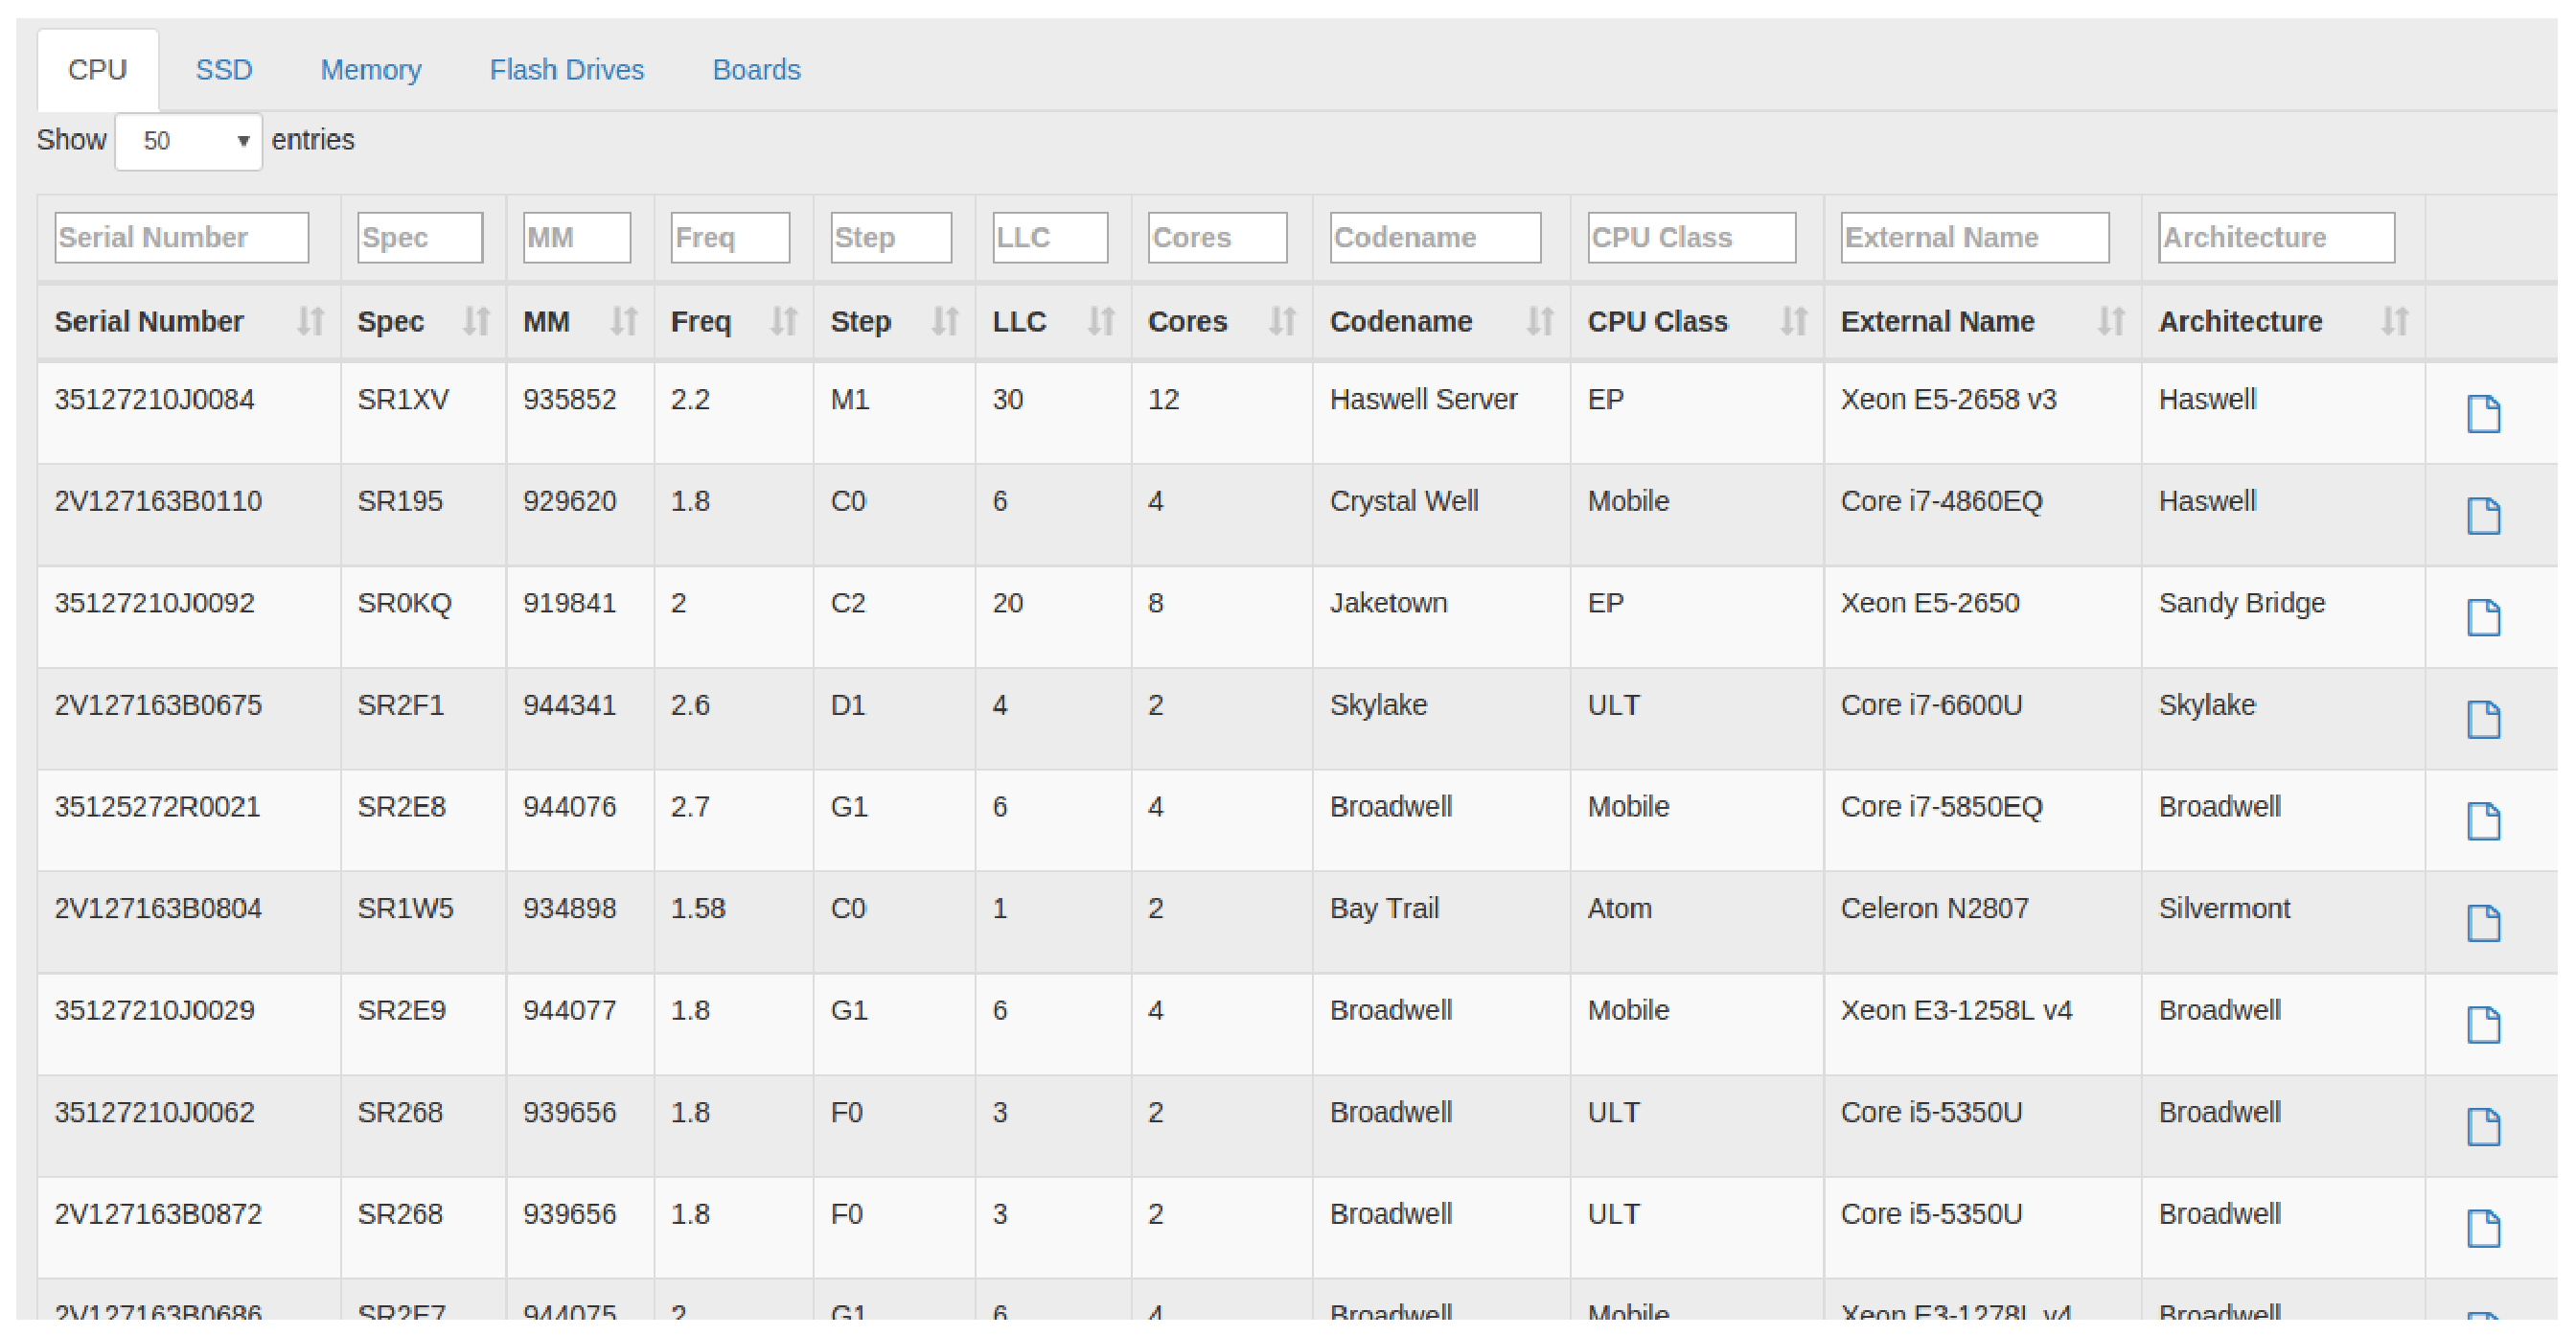
\includegraphics[width=0.9\textwidth]{img-4.eps}
    \caption{The CPU table.}
\end{figure}

\begin{figure}[!ht]
    \centering
    \captionsetup{justification=centering}
    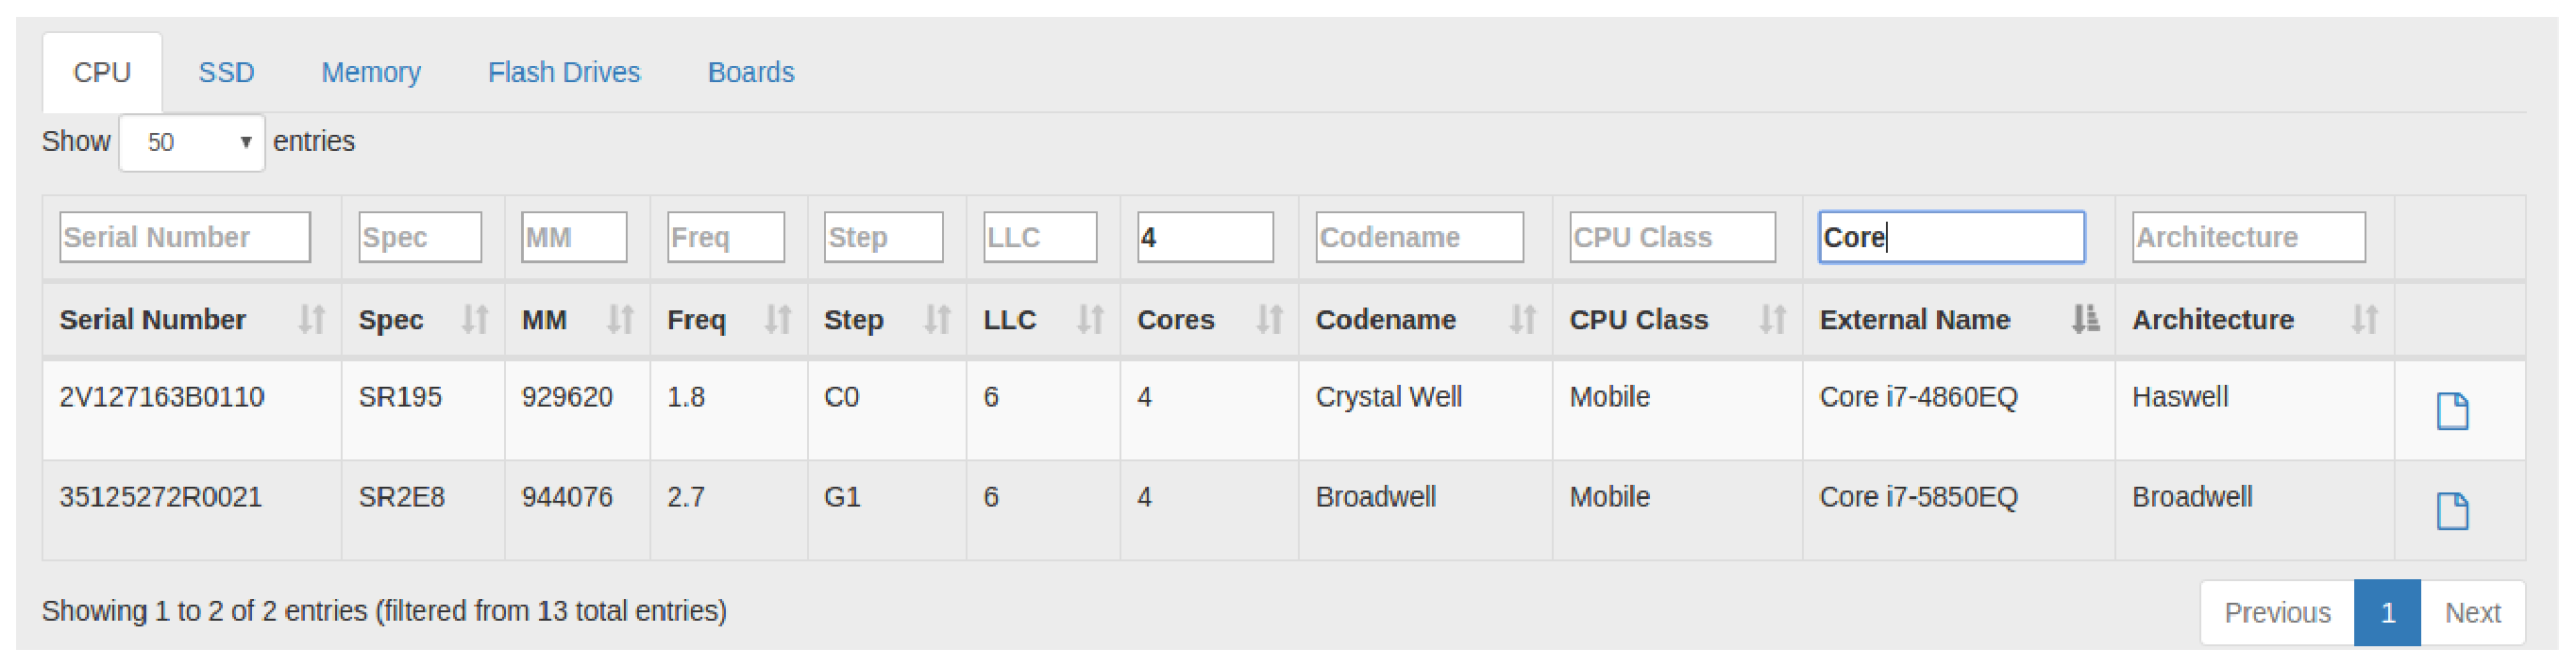
\includegraphics[width=0.9\textwidth]{img-3.eps}
    \caption{Filtering table based on number of cores and external name.}
\end{figure}

\begin{figure}[!ht]
    \centering
    \captionsetup{justification=centering}
    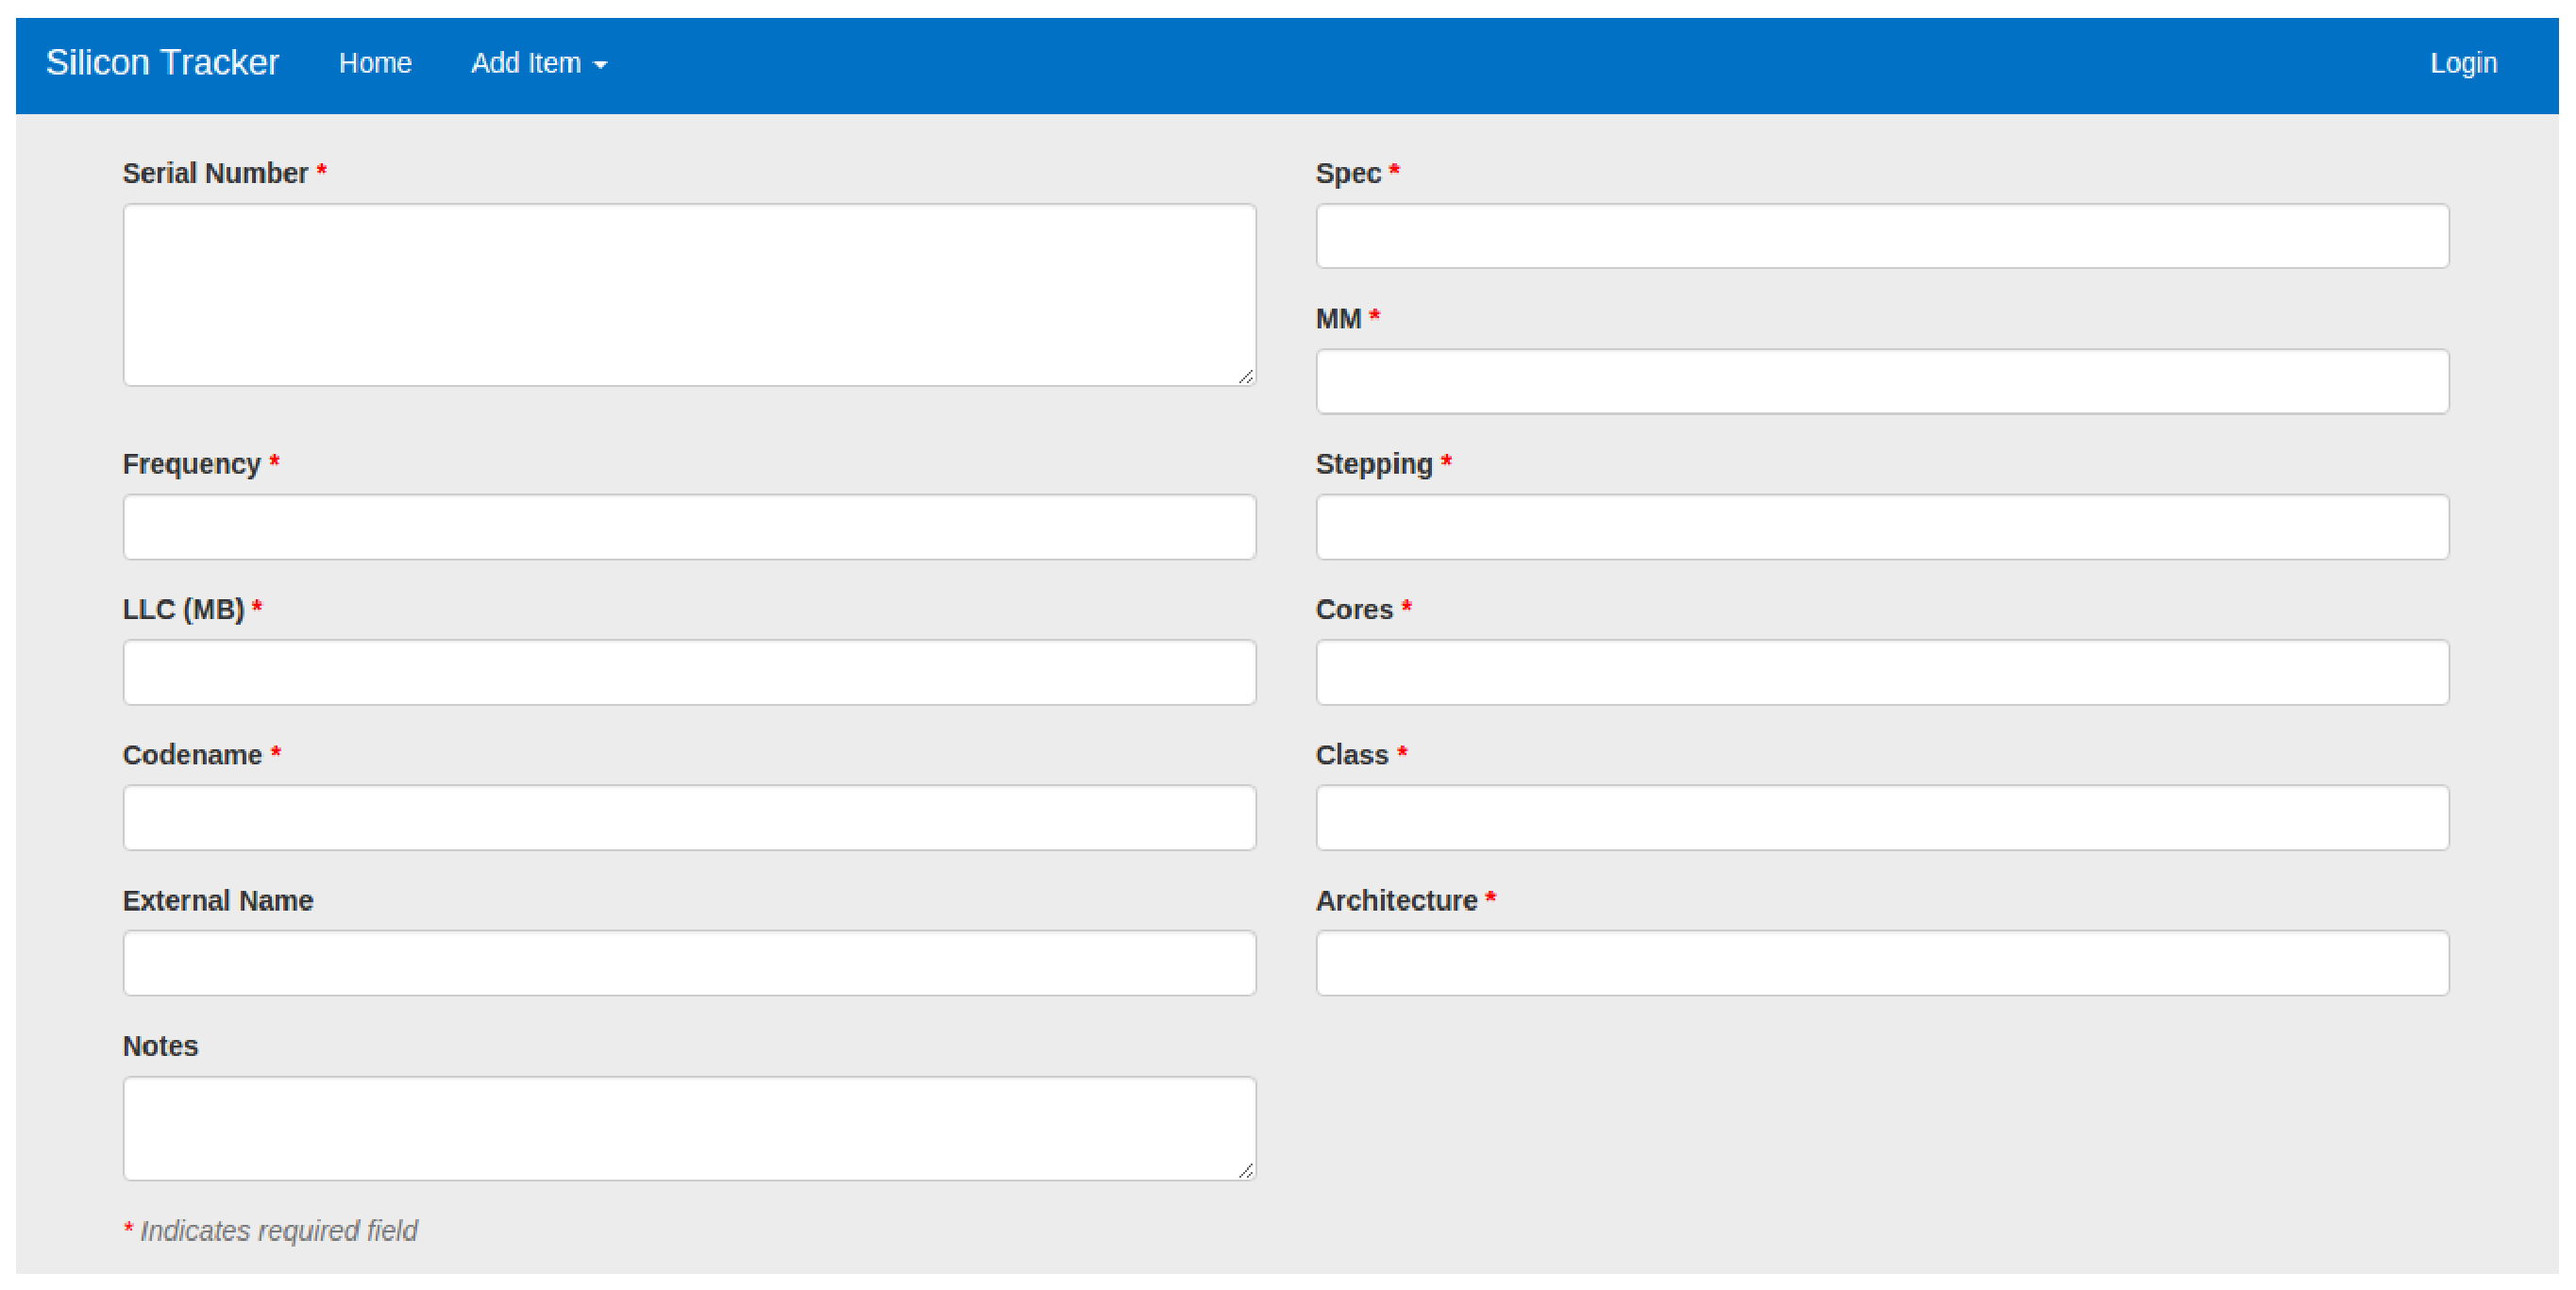
\includegraphics[width=0.9\textwidth]{img-2.eps}
    \caption{The screen for adding a new CPU.}
\end{figure}

\begin{figure}[!ht]
    \centering
    \captionsetup{justification=centering}
    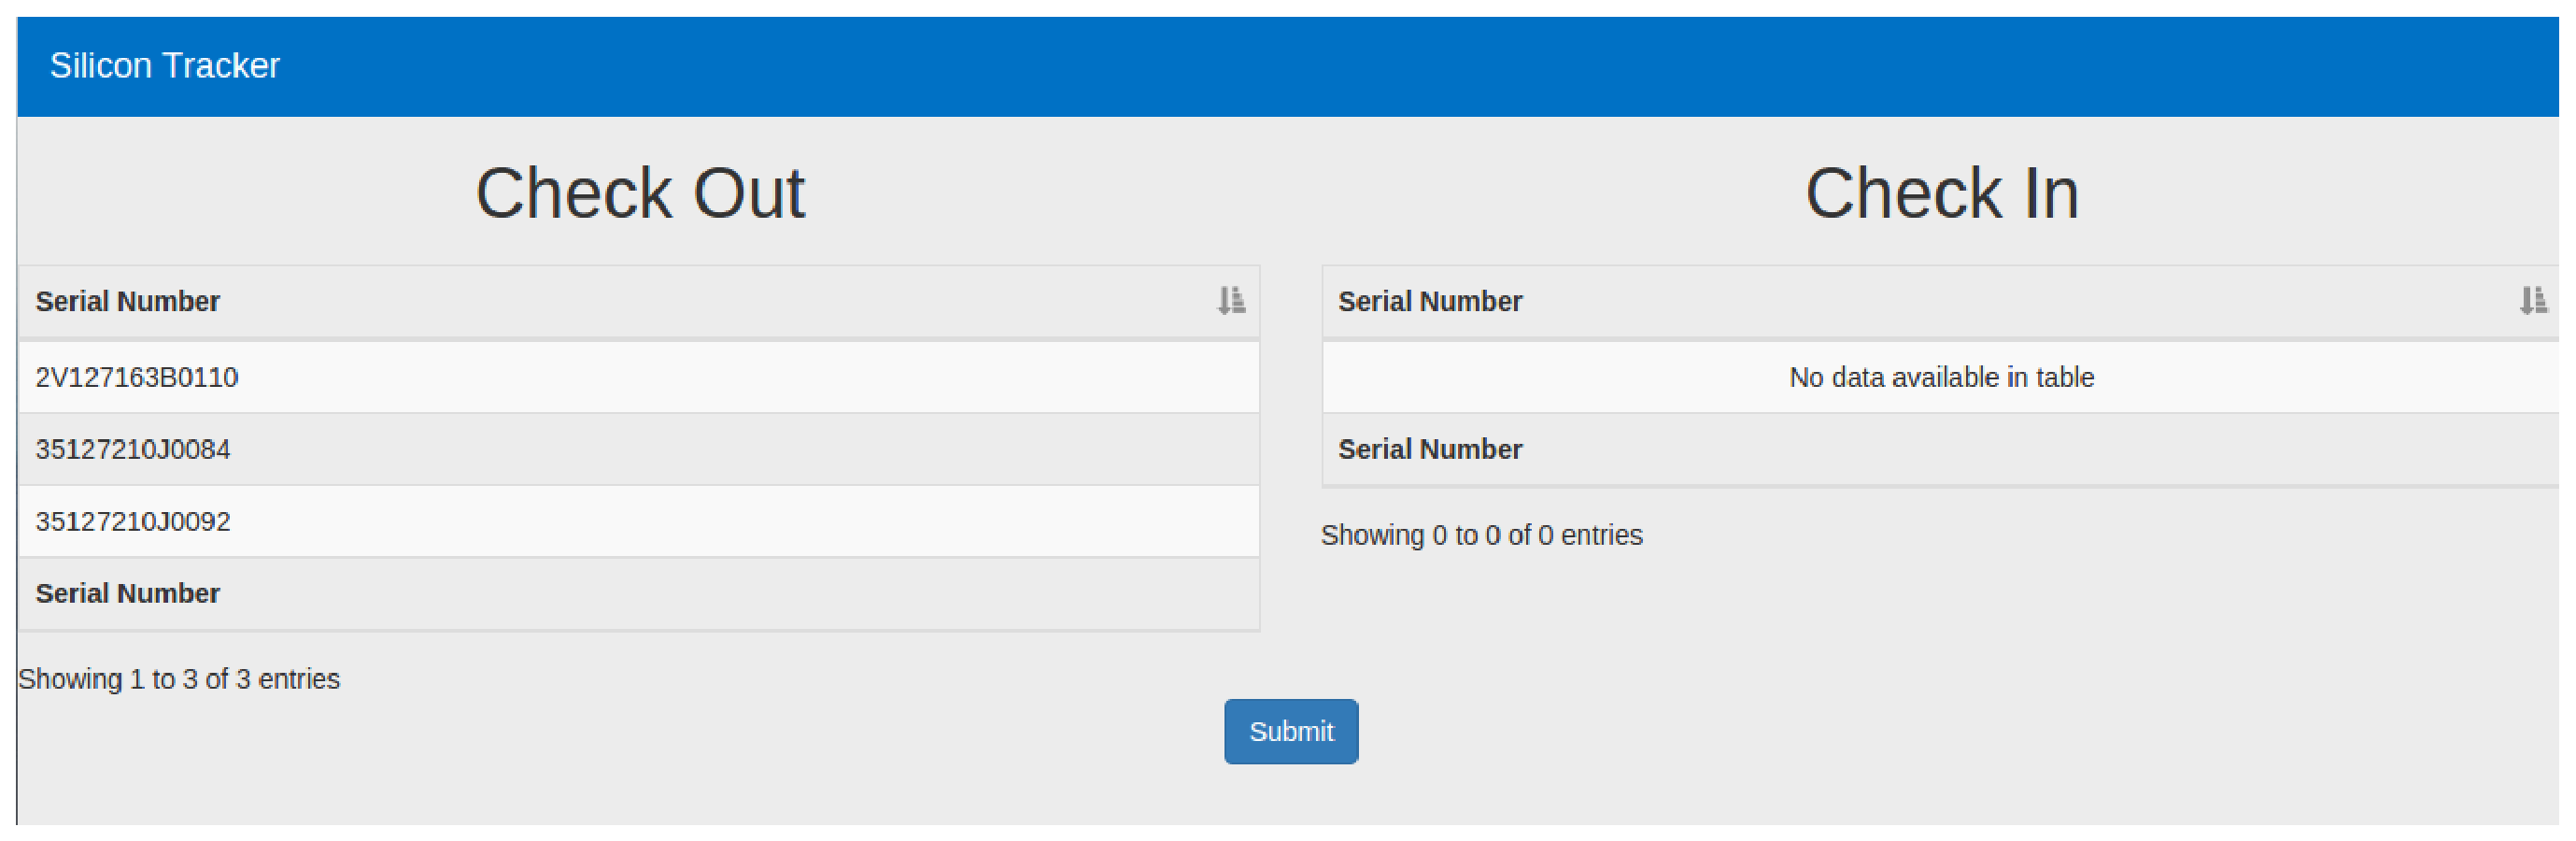
\includegraphics[width=0.9\textwidth]{img-1.eps}
    \caption{The kiosk cart screen, with some items to check out.}
\end{figure}


% needed in second column of first page if using \IEEEpubid
%\IEEEpubidadjcol

% \subsubsection{Subsubsection Heading Here}
% Subsubsection text here.


% An example of a floating figure using the graphicx package.
% Note that \label must occur AFTER (or within) \caption.
% For figures, \caption should occur after the \includegraphics.
% Note that IEEEtran v1.7 and later has special internal code that
% is designed to preserve the operation of \label within \caption
% even when the captionsoff option is in effect. However, because
% of issues like this, it may be the safest practice to put all your
% \label just after \caption rather than within \caption{}.
%
% Reminder: the "draftcls" or "draftclsnofoot", not "draft", class
% option should be used if it is desired that the figures are to be
% displayed while in draft mode.
%
%\begin{figure}[!t]
%\centering
%\includegraphics[width=2.5in]{myfigure}
% where an .eps filename suffix will be assumed under latex, 
% and a .pdf suffix will be assumed for pdflatex; or what has been declared
% via \DeclareGraphicsExtensions.
%\caption{Simulation results for the network.}
%\label{fig_sim}
%\end{figure}

% Note that the IEEE typically puts floats only at the top, even when this
% results in a large percentage of a column being occupied by floats.


% An example of a double column floating figure using two subfigures.
% (The subfig.sty package must be loaded for this to work.)
% The subfigure \label commands are set within each subfloat command,
% and the \label for the overall figure must come after \caption.
% \hfil is used as a separator to get equal spacing.
% Watch out that the combined width of all the subfigures on a 
% line do not exceed the text width or a line break will occur.
%
%\begin{figure*}[!t]
%\centering
%\subfloat[Case I]{\includegraphics[width=2.5in]{box}%
%\label{fig_first_case}}
%\hfil
%\subfloat[Case II]{\includegraphics[width=2.5in]{box}%
%\label{fig_second_case}}
%\caption{Simulation results for the network.}
%\label{fig_sim}
%\end{figure*}
%
% Note that often IEEE papers with subfigures do not employ subfigure
% captions (using the optional argument to \subfloat[]), but instead will
% reference/describe all of them (a), (b), etc., within the main caption.
% Be aware that for subfig.sty to generate the (a), (b), etc., subfigure
% labels, the optional argument to \subfloat must be present. If a
% subcaption is not desired, just leave its contents blank,
% e.g., \subfloat[].


% An example of a floating table. Note that, for IEEE style tables, the
% \caption command should come BEFORE the table and, given that table
% captions serve much like titles, are usually capitalized except for words
% such as a, an, and, as, at, but, by, for, in, nor, of, on, or, the, to
% and up, which are usually not capitalized unless they are the first or
% last word of the caption. Table text will default to \footnotesize as
% the IEEE normally uses this smaller font for tables.
% The \label must come after \caption as always.
%
%\begin{table}[!t]
%% increase table row spacing, adjust to taste
%\renewcommand{\arraystretch}{1.3}
% if using array.sty, it might be a good idea to tweak the value of
% \extrarowheight as needed to properly center the text within the cells
%\caption{An Example of a Table}
%\label{table_example}
%\centering
%% Some packages, such as MDW tools, offer better commands for making tables
%% than the plain LaTeX2e tabular which is used here.
%\begin{tabular}{|c||c|}
%\hline
%One & Two\\
%\hline
%Three & Four\\
%\hline
%\end{tabular}
%\end{table}


% Note that the IEEE does not put floats in the very first column
% - or typically anywhere on the first page for that matter. Also,
% in-text middle ("here") positioning is typically not used, but it
% is allowed and encouraged for Computer Society conferences (but
% not Computer Society journals). Most IEEE journals/conferences use
% top floats exclusively. 
% Note that, LaTeX2e, unlike IEEE journals/conferences, places
% footnotes above bottom floats. This can be corrected via the
% \fnbelowfloat command of the stfloats package.




% \section{Conclusion}
% The conclusion goes here.





% if have a single appendix:
%\appendix[Proof of the Zonklar Equations]
% or
%\appendix  % for no appendix heading
% do not use \section anymore after \appendix, only \section*
% is possibly needed

% use appendices with more than one appendix
% then use \section to start each appendix
% you must declare a \section before using any
% \subsection or using \label (\appendices by itself
% starts a section numbered zero.)
%


% \appendices
% \section{Proof of the First Zonklar Equation}
% Appendix one text goes here.

% you can choose not to have a title for an appendix
% if you want by leaving the argument blank
% \section{}
% Appendix two text goes here.


% use section* for acknowledgment
% \section*{Acknowledgment}


% The authors would like to thank...


% Can use something like this to put references on a page
% by themselves when using endfloat and the captionsoff option.
\ifCLASSOPTIONcaptionsoff
  \newpage
\fi



% trigger a \newpage just before the given reference
% number - used to balance the columns on the last page
% adjust value as needed - may need to be readjusted if
% the document is modified later
%\IEEEtriggeratref{8}
% The "triggered" command can be changed if desired:
%\IEEEtriggercmd{\enlargethispage{-5in}}

% references section

% can use a bibliography generated by BibTeX as a .bbl file
% BibTeX documentation can be easily obtained at:
% http://mirror.ctan.org/biblio/bibtex/contrib/doc/
% The IEEEtran BibTeX style support page is at:
% http://www.michaelshell.org/tex/ieeetran/bibtex/
%\bibliographystyle{IEEEtran}
% argument is your BibTeX string definitions and bibliography database(s)
%\bibliography{IEEEabrv,../bib/paper}
%
% <OR> manually copy in the resultant .bbl file
% set second argument of \begin to the number of references
% (used to reserve space for the reference number labels box)
% \begin{thebibliography}{1}

% \bibitem{IEEEhowto:kopka}
% H.~Kopka and P.~W. Daly, \emph{A Guide to \LaTeX}, 3rd~ed.\hskip 1em plus
%   0.5em minus 0.4em\relax Harlow, England: Addison-Wesley, 1999.

% \end{thebibliography}

% biography section
% 
% If you have an EPS/PDF photo (graphicx package needed) extra braces are
% needed around the contents of the optional argument to biography to prevent
% the LaTeX parser from getting confused when it sees the complicated
% \includegraphics command within an optional argument. (You could create
% your own custom macro containing the \includegraphics command to make things
% simpler here.)
%\begin{IEEEbiography}[{\includegraphics[width=1in,height=1.25in,clip,keepaspectratio]{mshell}}]{Michael Shell}
% or if you just want to reserve a space for a photo:

% \begin{IEEEbiography}{Michael Shell}
% Biography text here.
% \end{IEEEbiography}

% if you will not have a photo at all:
% \begin{IEEEbiographynophoto}{John Doe}
% Biography text here.
% \end{IEEEbiographynophoto}

% insert where needed to balance the two columns on the last page with
% biographies
%\newpage

% \begin{IEEEbiographynophoto}{Jane Doe}
% Biography text here.
% \end{IEEEbiographynophoto}

% You can push biographies down or up by placing
% a \vfill before or after them. The appropriate
% use of \vfill depends on what kind of text is
% on the last page and whether or not the columns
% are being equalized.

%\vfill

% Can be used to pull up biographies so that the bottom of the last one
% is flush with the other column.
%\enlargethispage{-5in}



% that's all folks
\end{document}


